\chapter{Main problems encountered during the work}
During the work some problems emerged, underlying the weak points that this approach might have. In this section we will focus on some of them to explain the overall problem analysed in a more complete way.

\section{A considerable amount of parameters}
The parameters involved in the optimization problem are not a small quantity, since this has to constantly take into consideration:
\begin{itemize}
  \item The number of eigenvalues being roots of the kernels polynomials;
  \item The value of $\sigma$ in the constraints, indicating the deviation around the $c$ value that the kernels could have;
  \item The number of non-root eigenvalues that has to be subject to the spectral constraints;
  \item The sparsity parameter;
  \item The number of iterations dedicated to the graph learning part and the number of them dedicated to the dictionary learning part;
\end{itemize}
This highlighted the need to spend some time on finding the right balance among them, in order for the linear programming solver to correctly go through the end and return a result without an unbounded objective function or infeasibility issues.

In this scenario, a particular attention was to be given to the $\sigma$ value, the number of root eigenvalues and to the number of non-root ones involved in the spectral constraints. We noticed that imposing them in a non proper way brought almost directly to an infeasibility issue, and if this was not encountered clearly at first, then it was simply hidden under an unbounded objective function problem.\\
When the process had to deal with infeasibility, of course the learned kernels were not reflecting the priors of the problems, resulting in weird behaviors, like the ones shown in \autoref{fig:kernelWeirdo} and for the $\alpha$ coefficients in \autoref{fig:alphaWeirdo}.

\begin{figure}
  \centering
  \begin{minipage}[c]{.8\textwidth}
    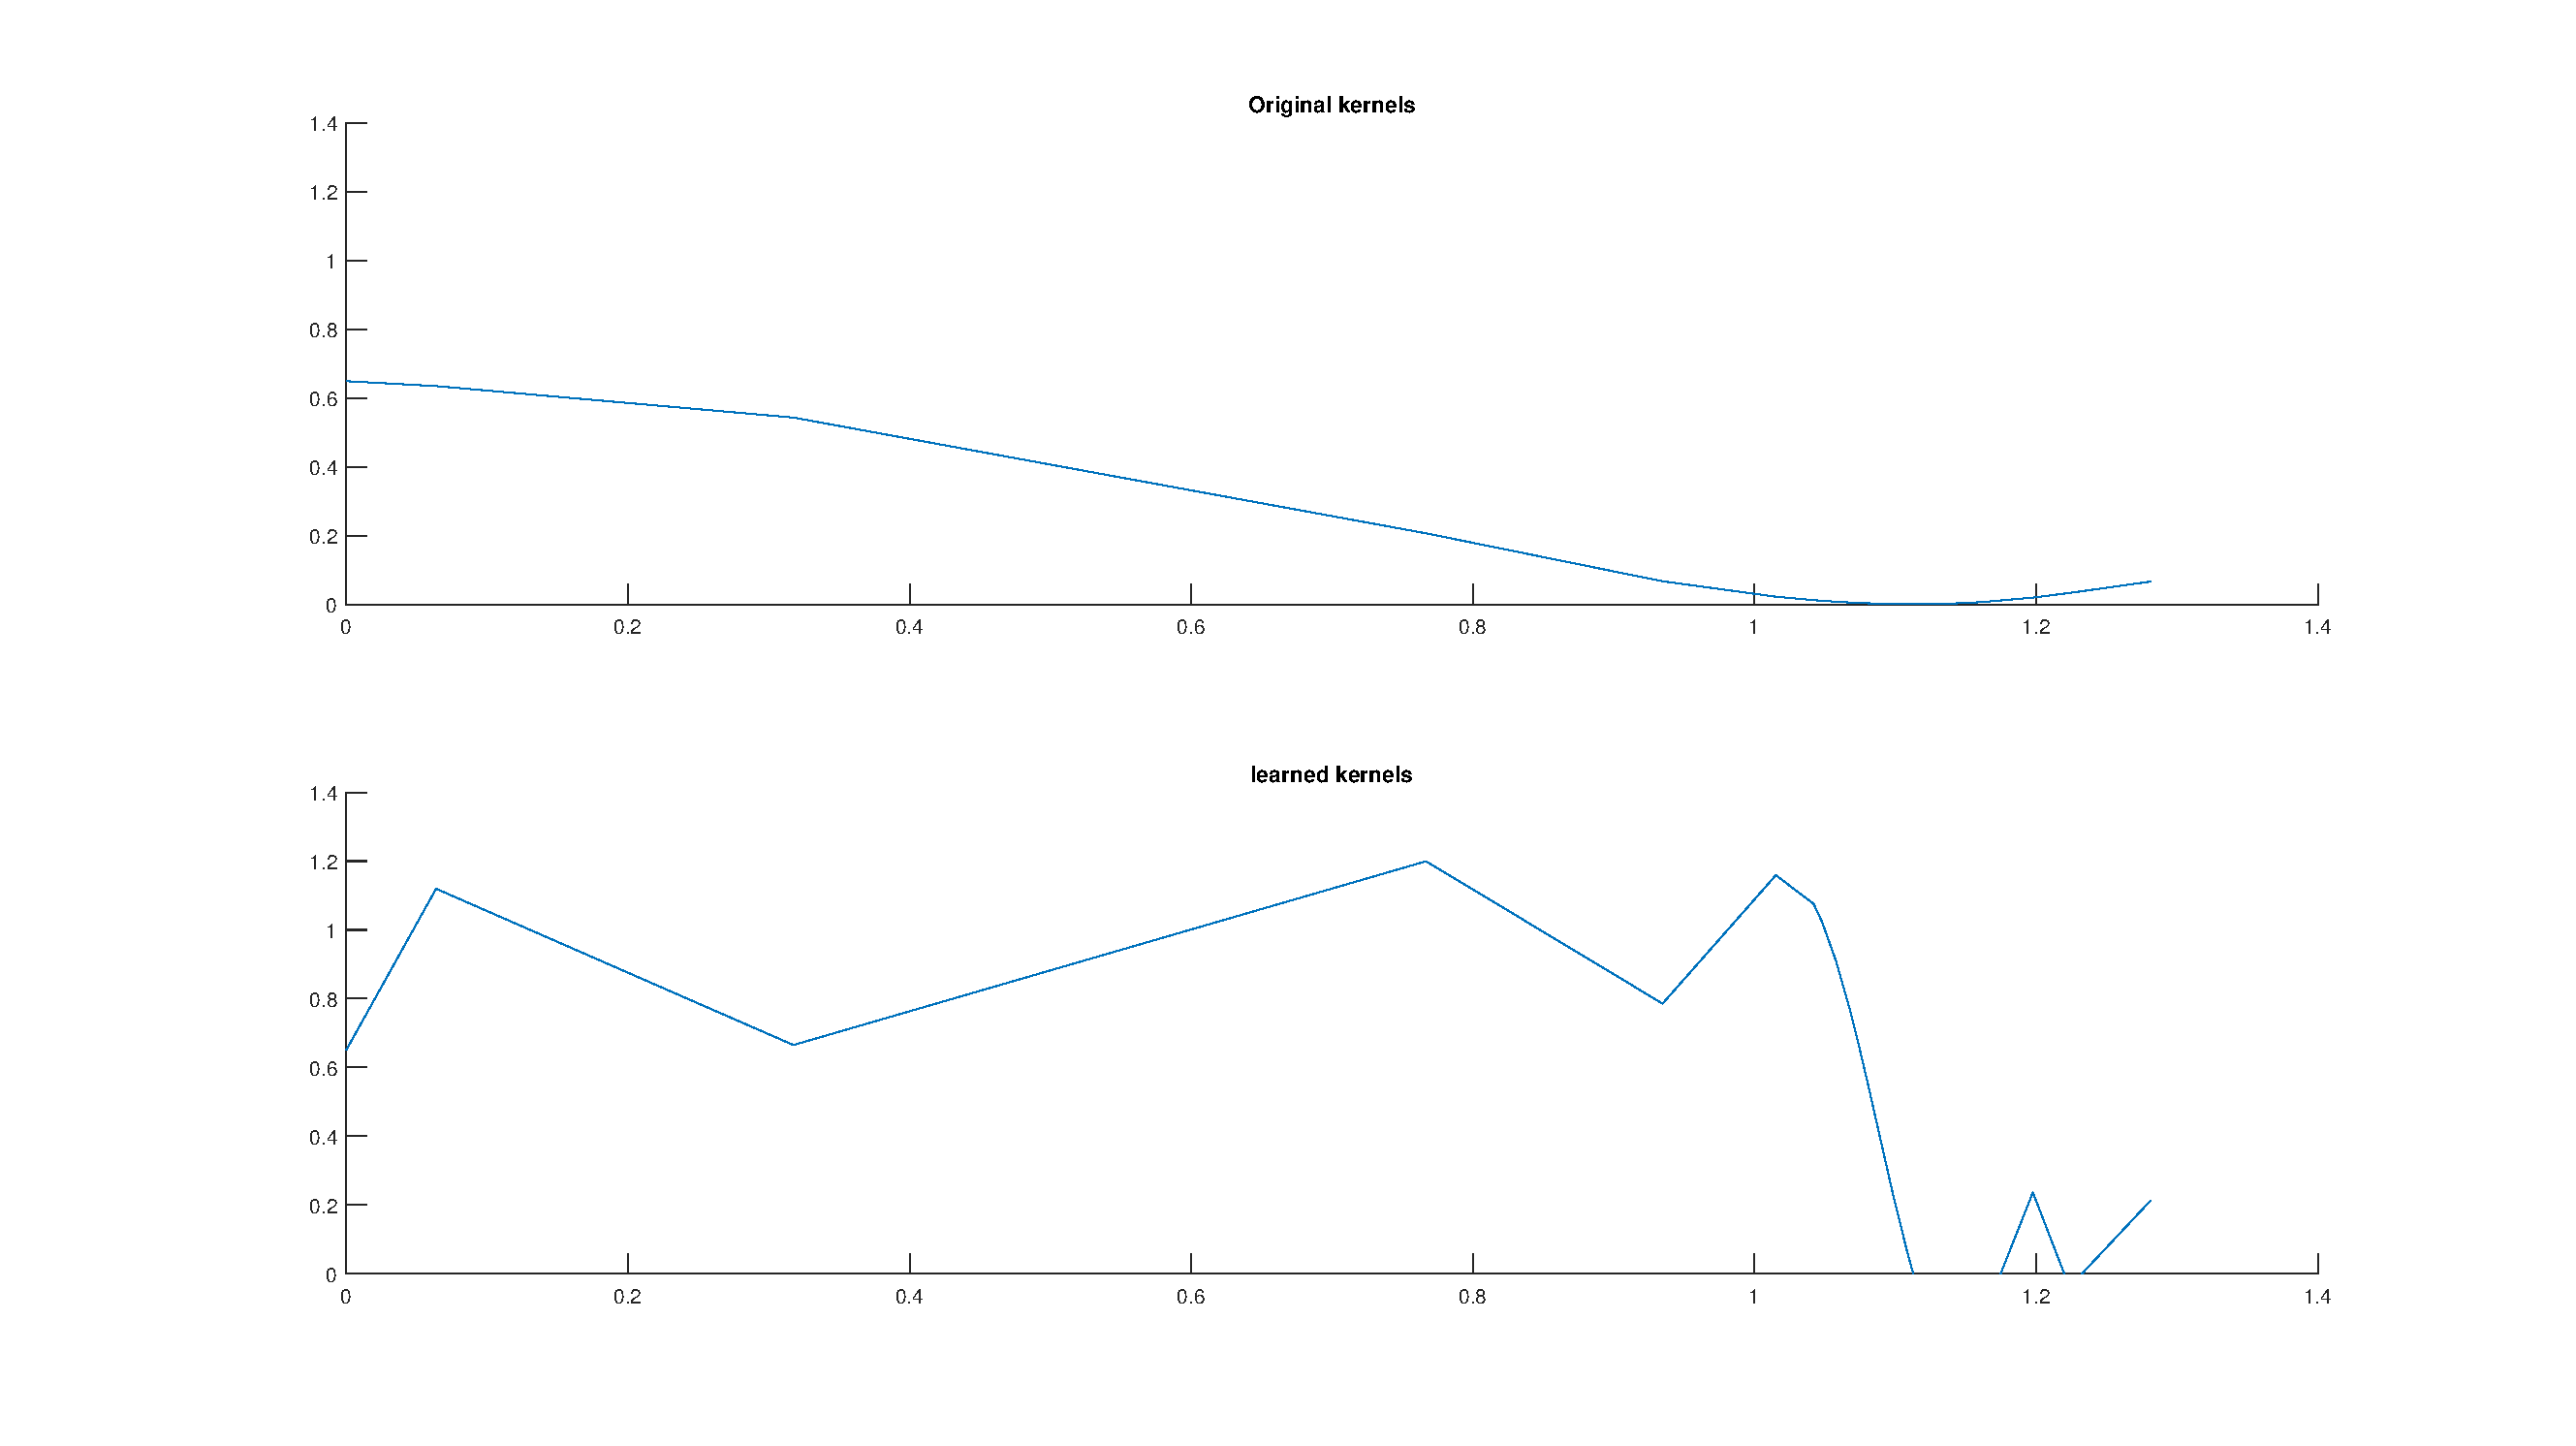
\includegraphics[width = \textwidth]{weirdoDorina.eps}
  \end{minipage}
  \begin{minipage}[c]{.8\textwidth}
    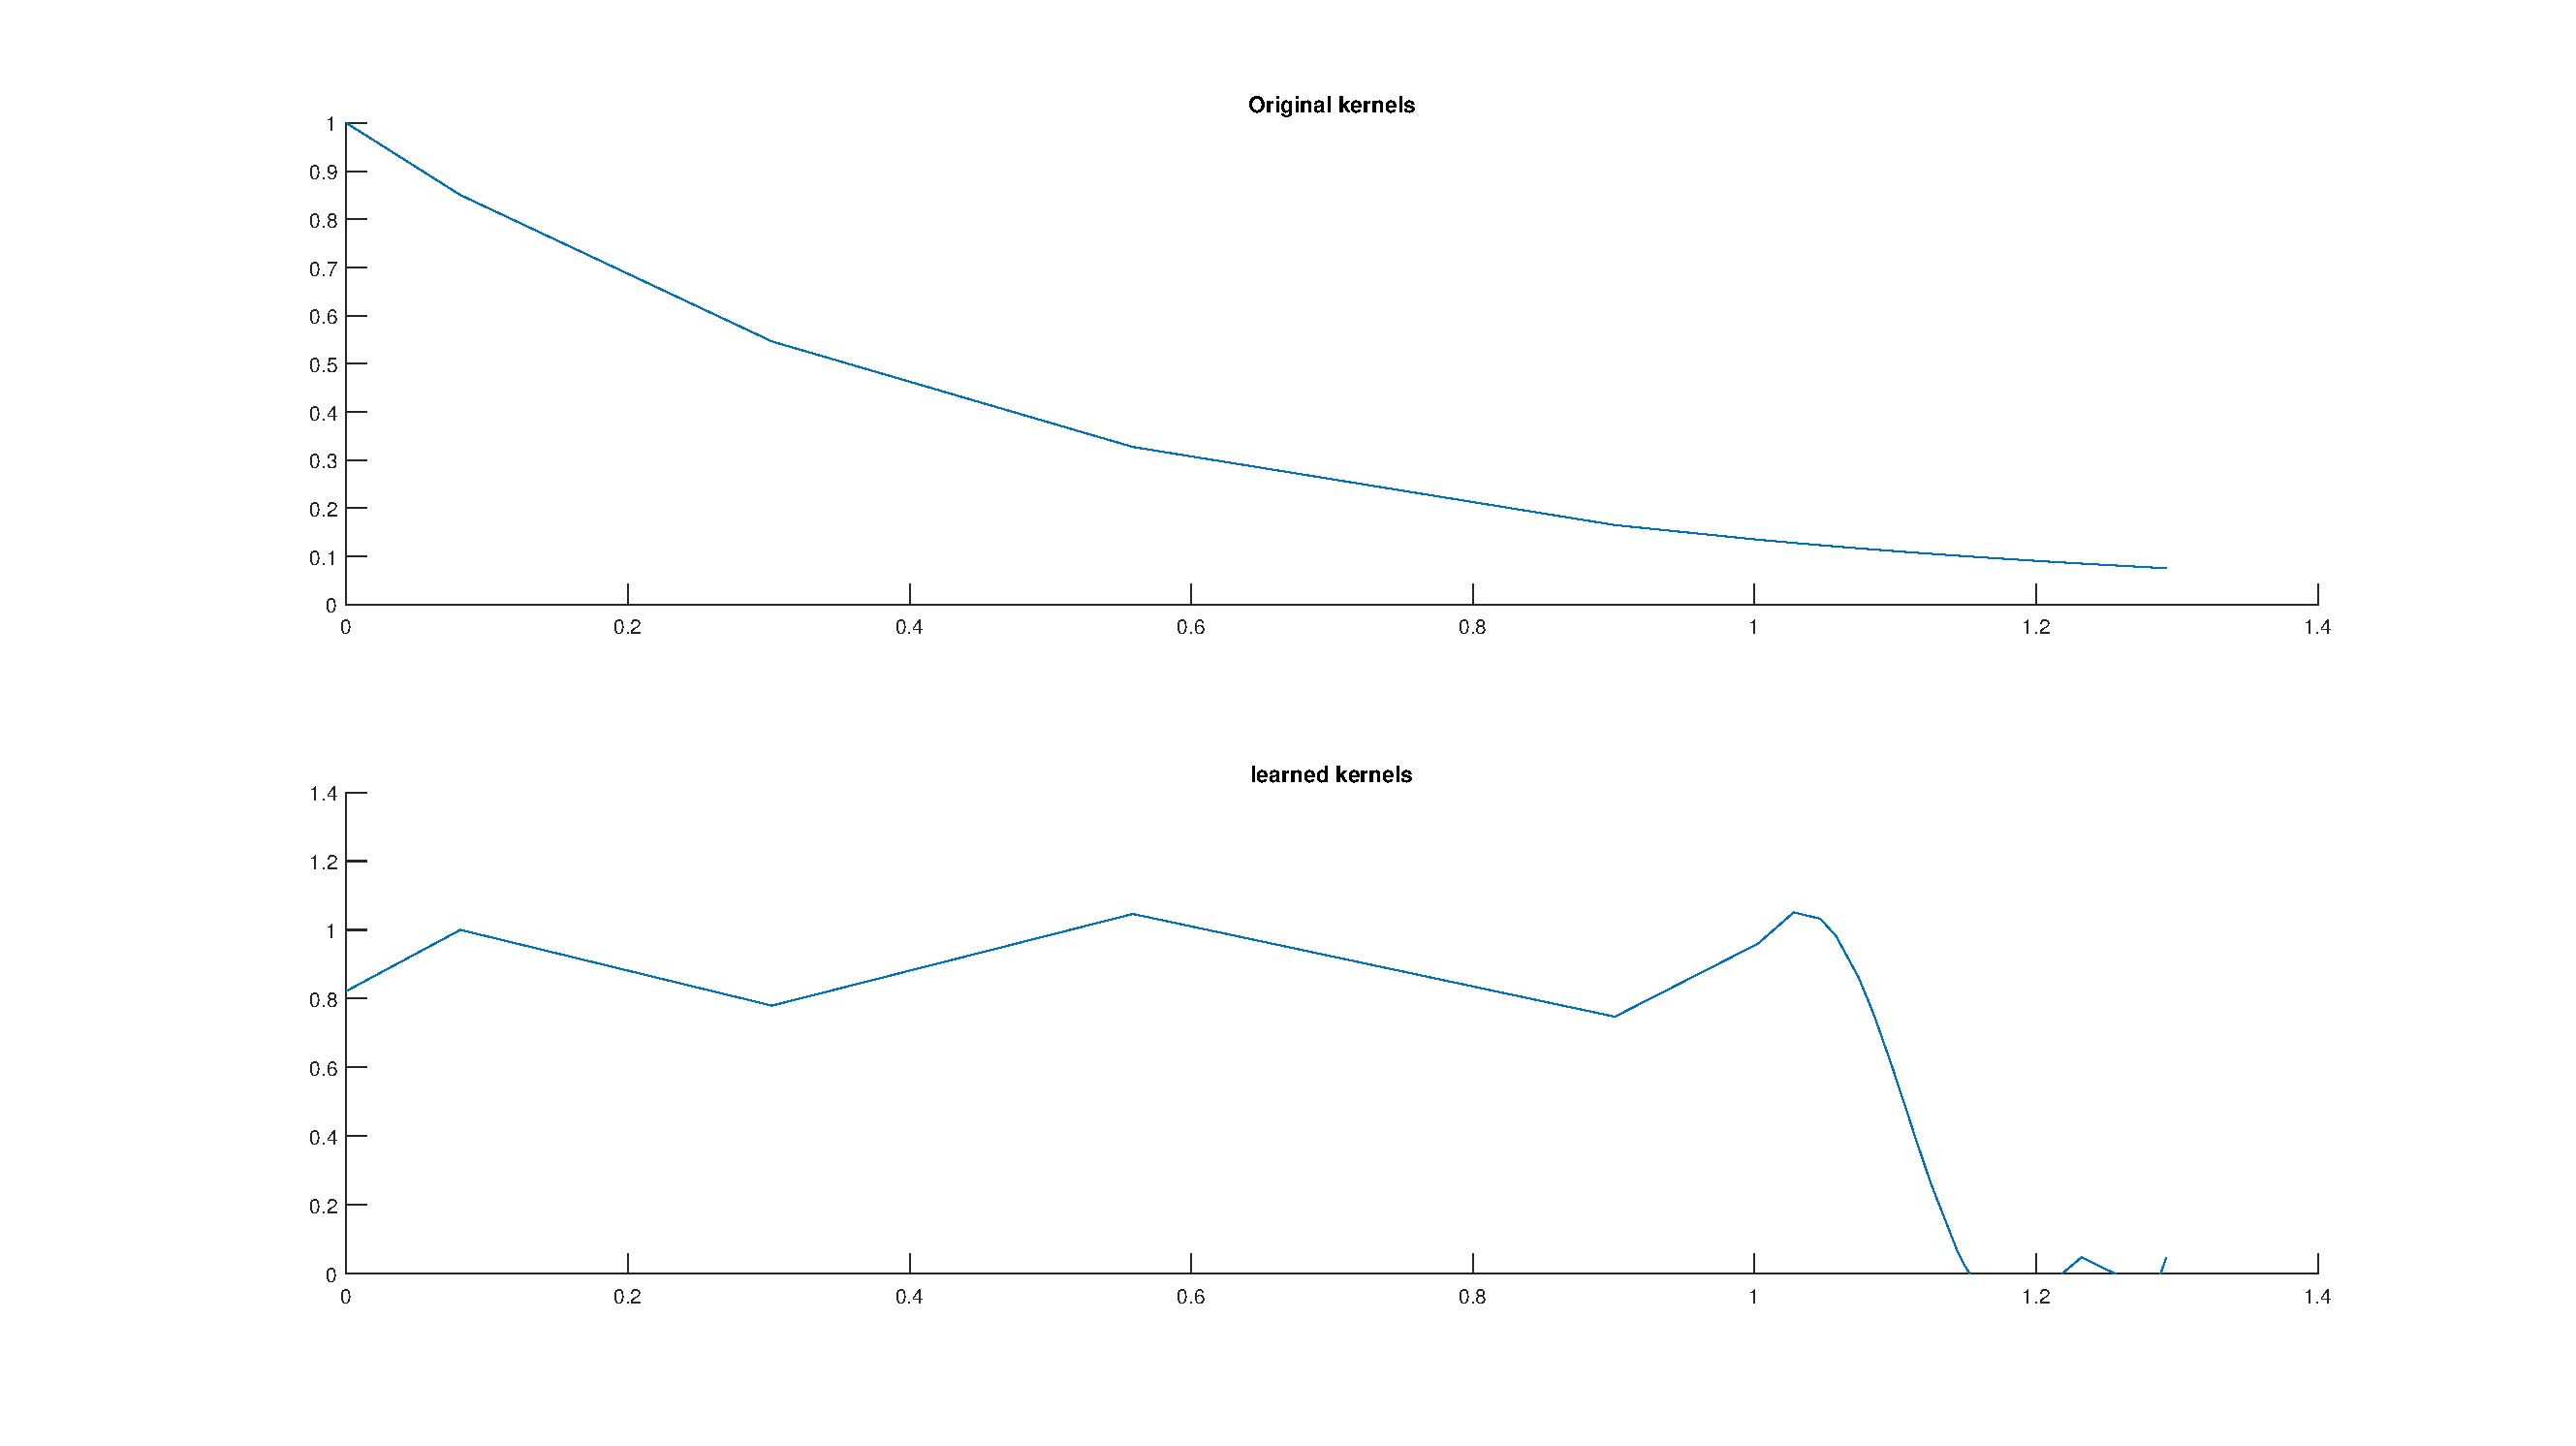
\includegraphics[width = \textwidth]{weirdoHeat.eps}
  \end{minipage}
  \caption{Comparison between the original kernel and the kernel learned with infeasibility problems}
  \label{fig:kernelWeirdo}
\end{figure}

\begin{figure}
  \centering
  \begin{minipage}[c]{.8\textwidth}
    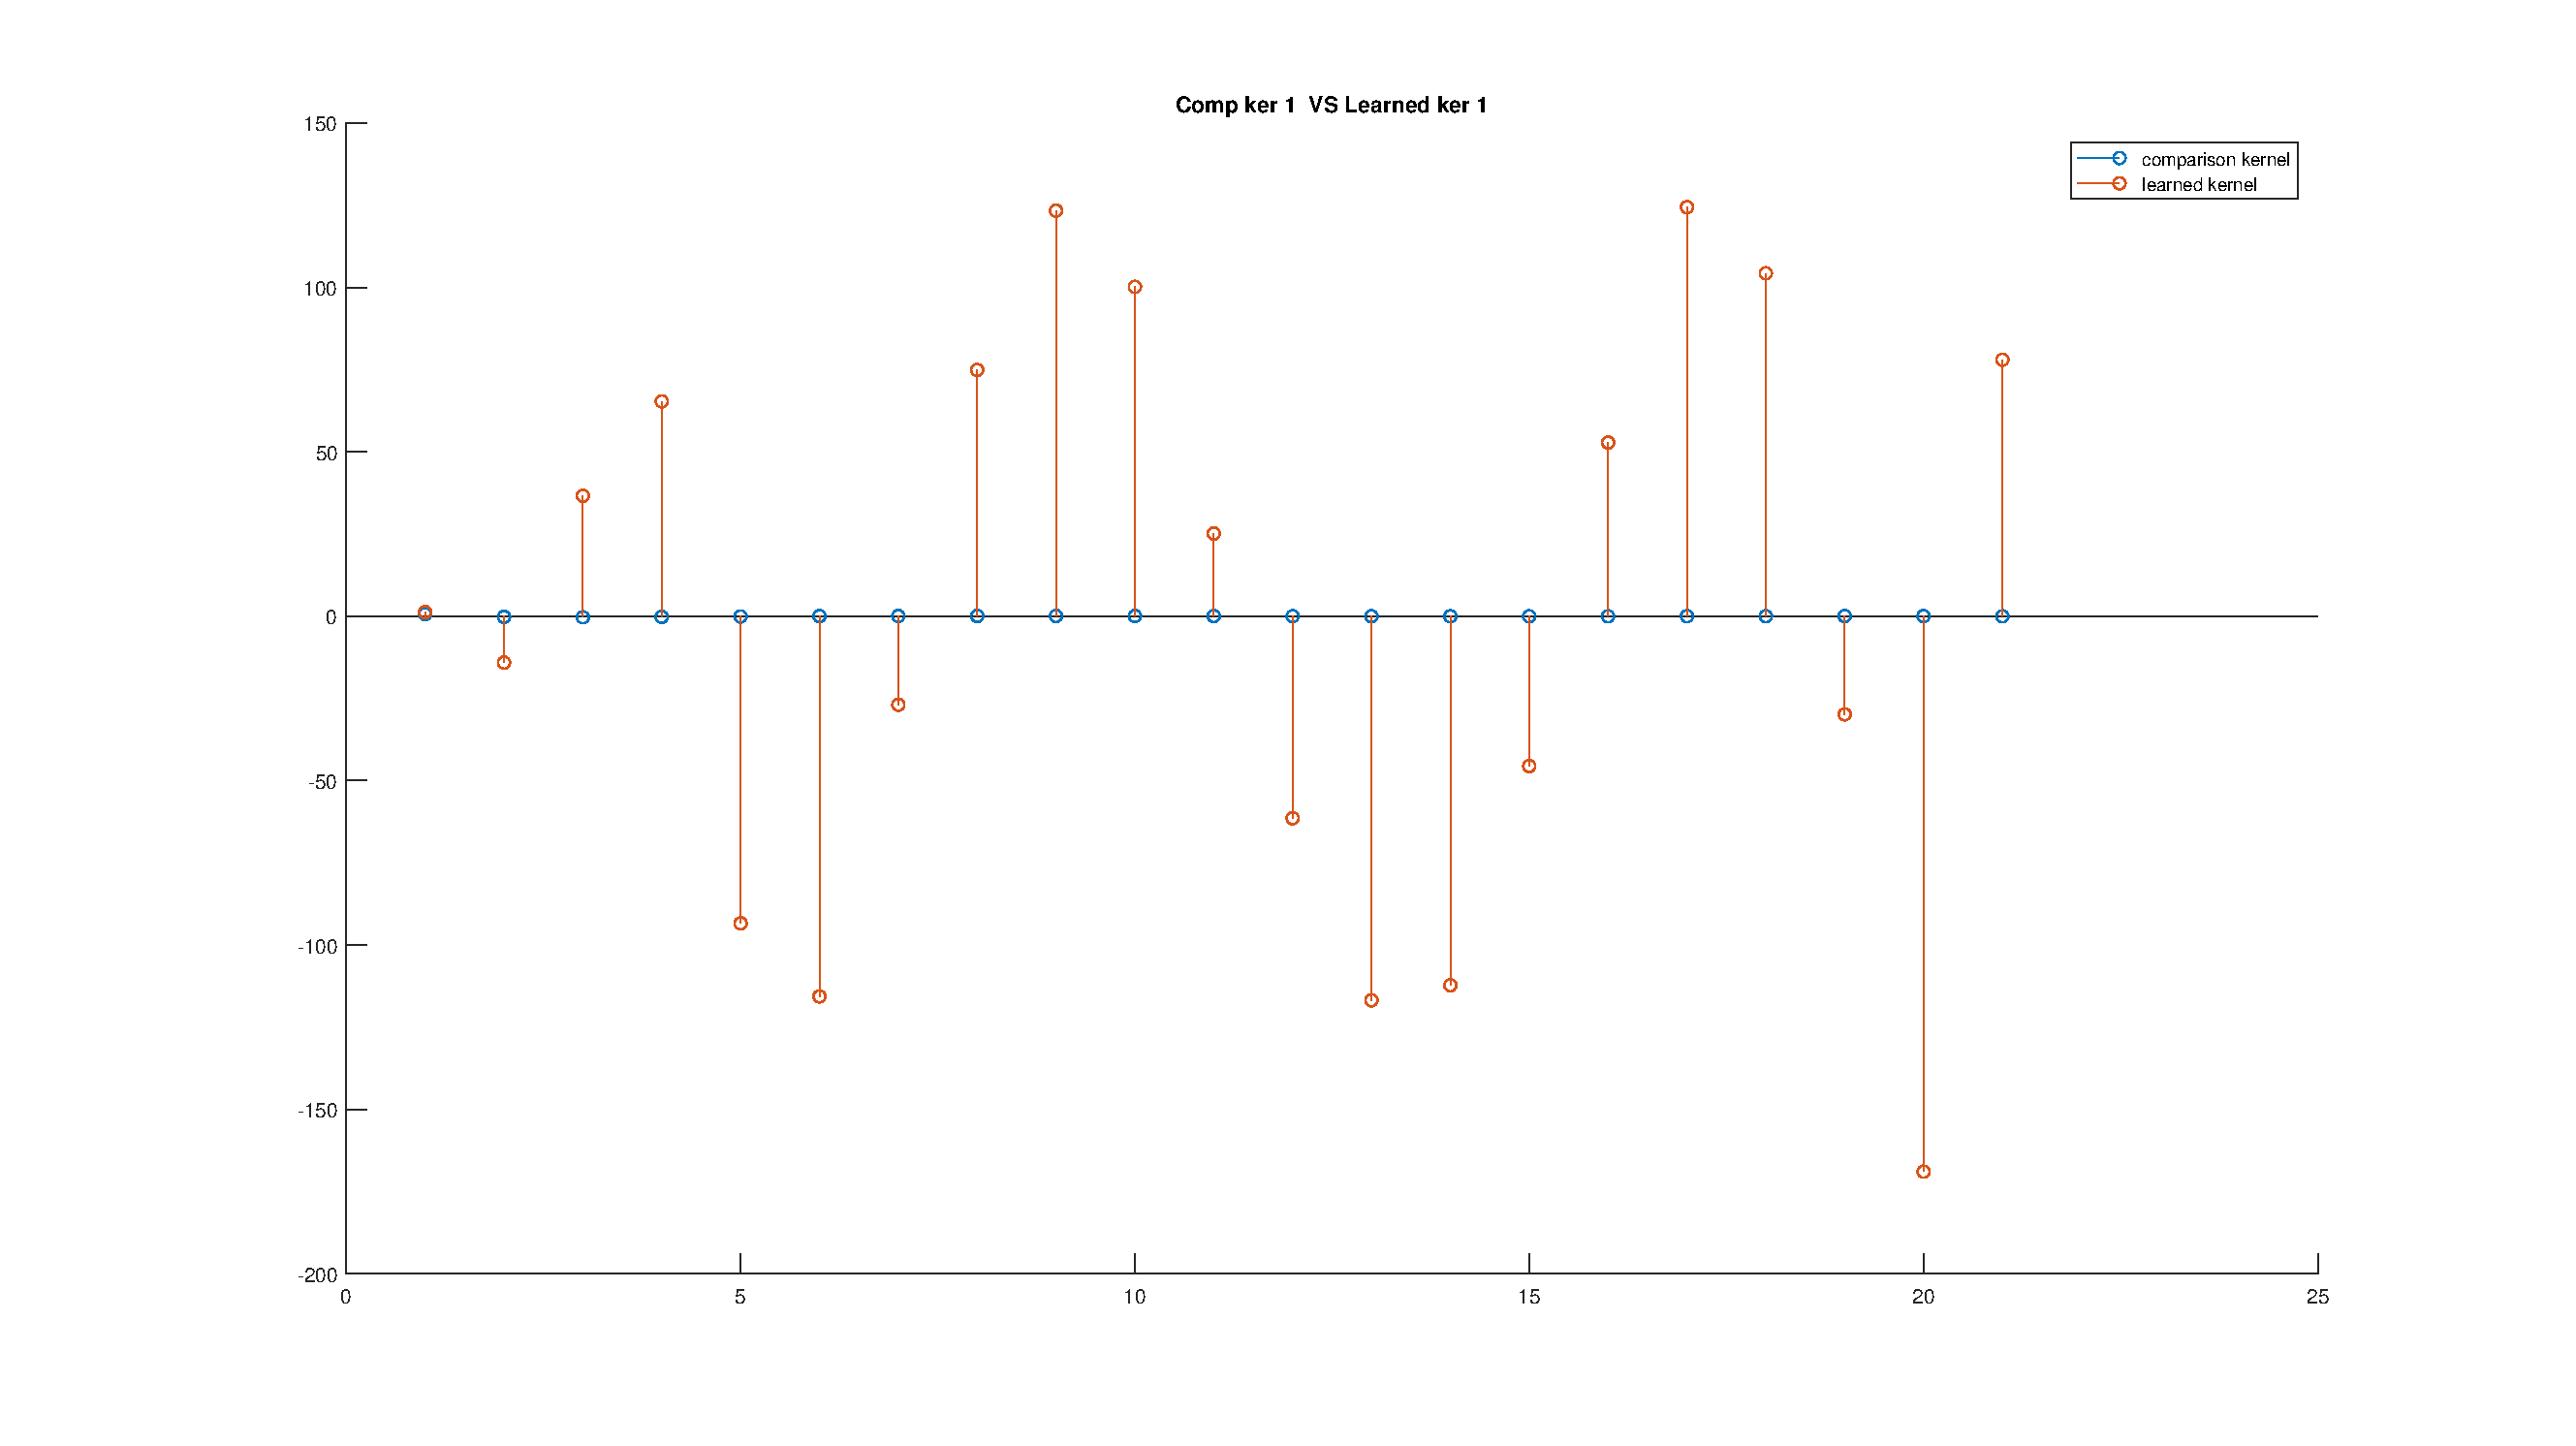
\includegraphics[width = \textwidth]{weirdoDorinaAlpha.eps}
  \end{minipage}
  \begin{minipage}[c]{.8\textwidth}
    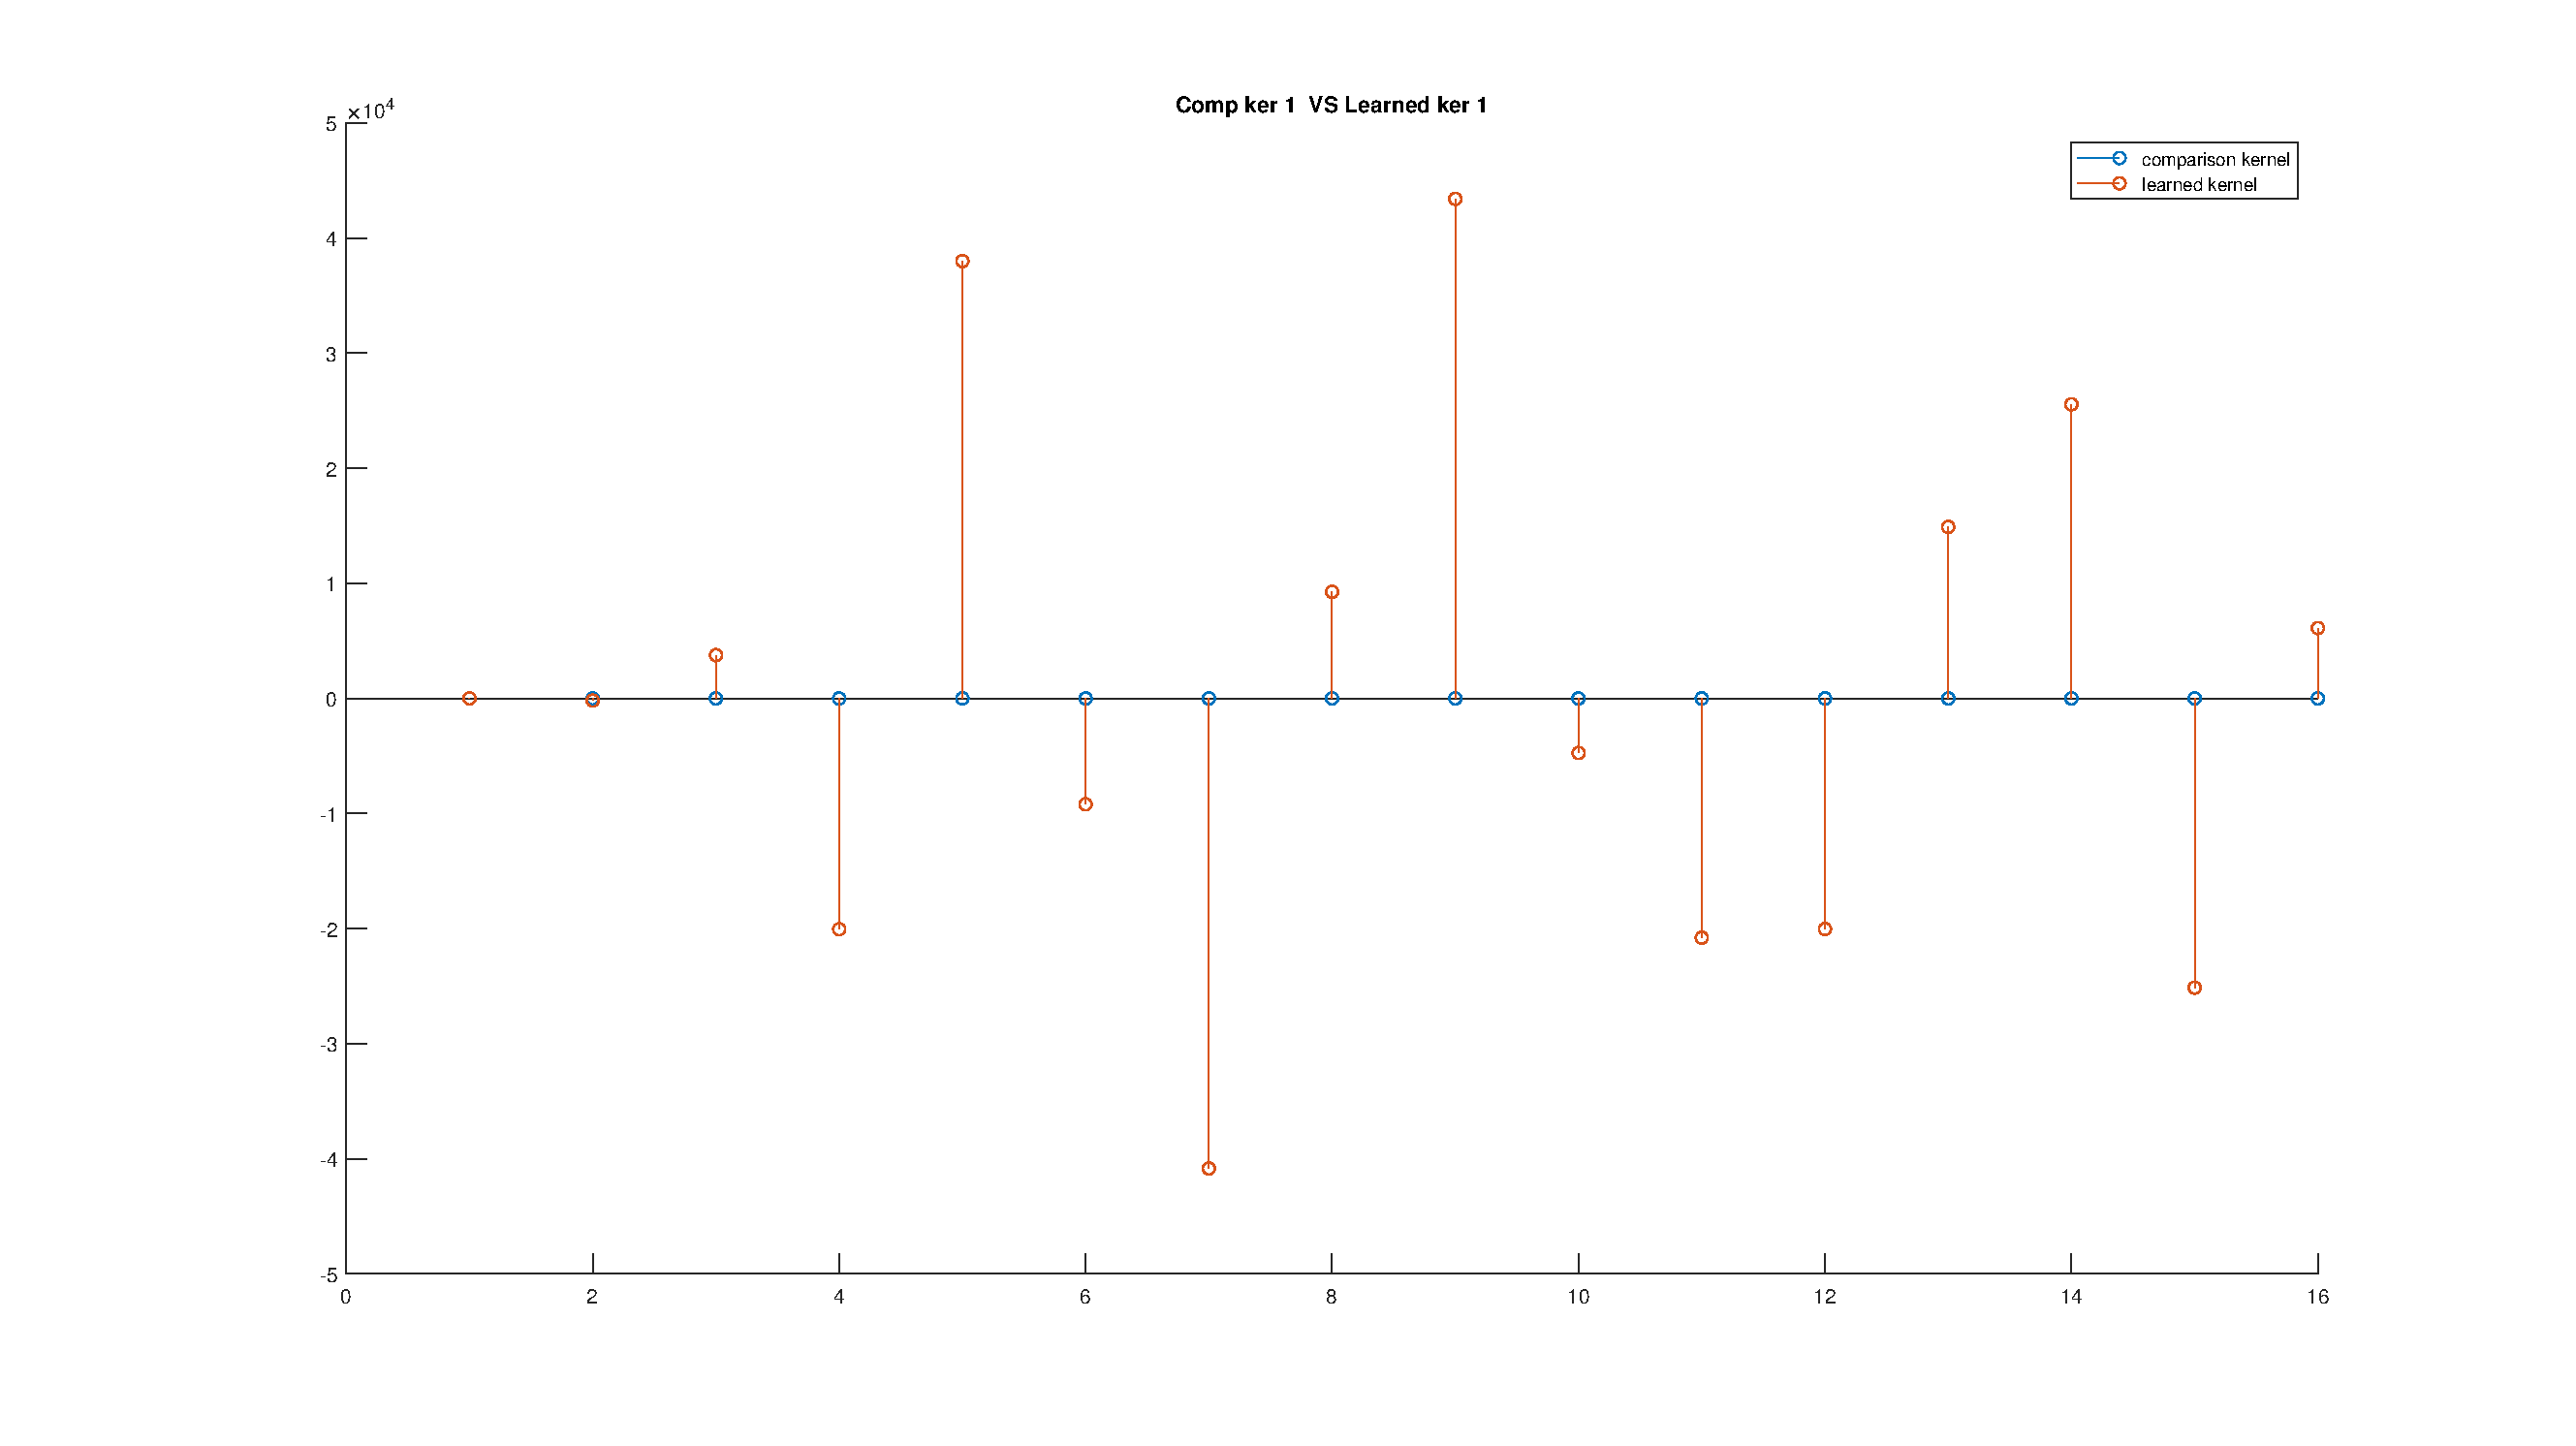
\includegraphics[width = \textwidth]{weirdoHeatAlpha.eps}
  \end{minipage}
  \caption{Comparison between the original $\alpha$ coefficients and the coefficients learned with infeasibility problems, for the Heat kernel and the synthetic dataset from Thanou et al.. It can be seen how now the learned $\alpha$s are several times bigger than the magnitude of the original coefficients, these ones resulting compressed around $0$ in the representation.}
  \label{fig:alphaWeirdo}
\end{figure}

% Another consequence of that was the output dictionary $\mathcal{D}$ and, accordingly, the sparsity matrix $X$: with infeasibility problems, in fact, the dictionary resulted in having very small values (even in the order of $10^{-8}$) while in a specular way the sparsity matrix was resulting in very high values in the non-zero element positions.\autoref{fig:dictionaryWeirdo} and \autoref{xWeirdo} show respectively the 3D-plot of the dictionary matrix and of the sparsity matrix, from them we can see the very small/high values the non-zero elements assume.
\cri{aggiungi foto di dizionario e sparsity matrix}
\cri{in realtà ora non ho più questi problemi...trova il modo di riottenerli}

\section{Working with the proper dataset}
The choice of the dataset has not been an easy task, first of all not many datasets are already set in such a way that we could use them in a plug and play manner. Other two datasets we used, as an alternative to the ones we already presented, were the complete synthetic one from Thanou et al. and a dataset collecting the number of Uber rides occurring in an area of Manhattan, grouped by hour and in different times of the day. There was also an attempt to extrapolate a coherent dataset from a group of photos stored in the Flickr database \cite{McAuley2012}, for example building a graph signal where the nodes were the locations of the pictures and the samples could have been the number of pictures taken from a single user in that location, repeated by the total number of users. This idea was later abandoned since the dataset obtained was not properly descriptive of the phenomena and the number of samples for the signal revealed to be insufficient for the training of the algorithm.\\

The problem with the other two datasets was the structure of the kernels: both Uber and the synthetic dataset were using not only low-frequency kernels, but also high frequency ones or even kernels having an ambiguous behavior, which can not be associated with either one (\autoref{fig:DorinaInBetween}). Therefore, in these cases we tried to modify the original signal in such a way that the learned dictionary could have returned only low frequency kernels. In particular, we tried to induce a well-know behavior either in the signal matrix or in the weight matrix, like for example through smoothing the values following a certain gradient, to see if we would have detected a precise response in the learned kernels' structure. However the trials did not bring to meaningful achievements or significative changes in the kernels such that we could extrapolate a pattern.
\cri{vedi se aggiungere plot di $W$ e $Y$ smussati, c'è una cosa super figa qui https://it.mathworks.com/help/matlab/ref/axes.html}

\begin{figure}[tb]
  \centering
  \includegraphics[width = 0.7\textwidth]{comp_kernels_dorina.png}
  \caption{The original kernels learned from the synthetic dataset of Thanou et al.. It can be seen how the orange kernel does not have a clear behavior in terms of high or low frequency}
  \label{fig:DorinaInBetween}
\end{figure}

\section{The peculiar structure of the kernels}
 In order to deploy at least the real dataset from Uber rides, we tried to extend our hypothesis so to see if there could be a general improvement of the learning frame not only imposing the smoothness on the kernels, but also forcing in the algorithm a more general structure in such a way that it was able to follow all the kernel behaviors. In the case of Uber dataset, for example, the dictionary learned involves one low frequency and one high frequency kernel, as can be seen in figure \ref{fig:uber}, and we consequently modified the algorithm in order for it to "filter" both of them on the high and low frequencies respectively. The results obtained, however, show that the smoothness one is a much more effective prior than its counterpart working on the high frequencies, and as a consequence the reproduction error was not reduced, but on the contrary was increasing.

 \begin{figure}[tb]
   \centering
   \includegraphics[width = 0.7\textwidth]{comp_kernels_Uber.png}
   \caption{The original kernels learned from the Uber dataset.}
   \label{fig:uber}
 \end{figure}

 \section{Relaxing the spectral constraints}
In order to make the optimization process more stable, we had to relax the constraints involved, in particular the spectral ones. At first we tried with relaxing and/or removing some of the bounds included in them in such a way: \cri{vai a sistemare il font della D nell'eq 1.4}
\begin{equation}
\mathcal{D}_s \succeq 0 \qquad \text{and} \qquad \sum_{s=1}^S\mathcal{D}_s \succeq 0
\end{equation}
But through it we observed an increased imprecision in the results, as expected, such that the smoothness prior was not being beneficial as we desire. At the same time, when restoring this bounds, we had to be careful in order to make them consistent with the new smoothness priors we added: we could not simply impose the last values of the kernels to be $0$ and in parallel require that all the other values were in a $(-\epsilon;+\epsilon)$ neighbourhood of $c$, since we would not have given the kernels the necessary margin to transition from that neighbourhood to $0$. The result of this lack was, of course, infeasibility.
